% Talk about PEP-II and its asymmetrical beam energies
PEP-II is an asymmetrical $e^- e^+$ collider at SLAC.
In PEP-II, $B$ mesons are produced primarily in the following process:
$e^- e^+ \rightarrow \Y4S/ \rightarrow B \bar{B}$, with
$e^-$ and $e^+$ beams tuned at different energies,
such that the invariant mass is at the \Y4S/ resonance (\SI{10.58}{GeV}),
and the momentum of the \Y4S/ in the lab frame
non-zero \cite{Harrison:1998yr}.

Producing at \Y4S/ peak leads to near-exclusive $B \bar{B}$ pair meson
production, reducing combinatorial background.
Also, since the momenta of $e^- e^+$ is known, with the reconstruction of the
momentum of one $B$ meson ($B_{tag}$), the momentum of the other $B$
($B_{sig}$) can be calculated as
\begin{equation}
    p_{B_{sig}} = p_{e^-e^+} - p_{B_{tag}}.
\end{equation}
Later we will see that knowing the exact $p_{B_{sig}}$ makes identifying events
that have more than one missing particle easier.

% Talk about subdetectors
\BaBar/ is a nearly $4\pi$ spetrometer (shown in
\autoref{fig:babar_detector_view}) that consists of five subdetectors.
From inside out:
Silicon Vertex Tracker (SVT) and Drift Chamber (DCH), which measure the momenta
and angles of charged particles with the help of a \SI{1.5}{T}.
Detector of Internally Reflected Cerenkov radiation (DIRC), together with SVT
and DCH, identifies charged particles of different masses by Cerenkov
ring-imaging and ionization energy loss of these particles.
Cesium Iodide Electromagnetic Calorimeter (EMC) measures energy and
position of electromagnetic showers generated by electrons and photons.
A superconducting solenoid with a \SI{1.5}{T} magnetic field surrounding the
EMC is part of the tracking and particle identification system which identifies
muons and some neutral hadrons together with Instrumented Flux Return
(IFR) \cite{Lees:2013uzd}.

\begin{figure}[ht]
    \centering
    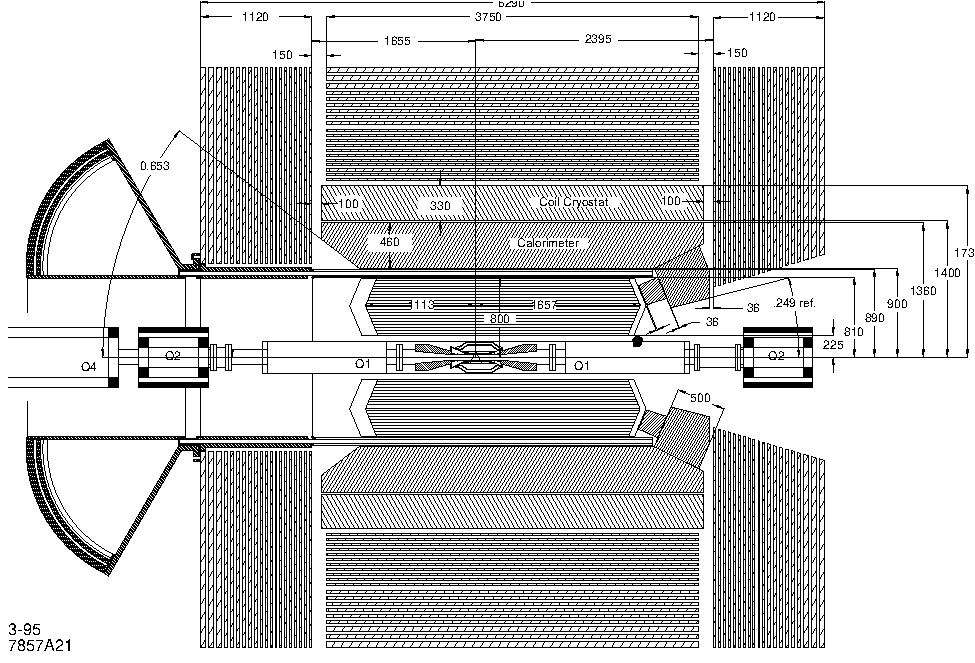
\includegraphics[width=0.7\textwidth]{figs/babar_detector_view.pdf}
    \caption{
        View of the \BaBar/ detector.
        Extracted from \cite{Boutigny:1995ib}.
    }
    \label{fig:babar_detector_view}
\end{figure}

% Talk about BaBar being 4 pi
At $B$ factories, $b \bar{b}$ are produced at all angles with
non-negligible probability \cite{Boutigny:1995ib,McGregor:2008ek}, thus the
detector needs to cover almost all solid angles (a $4\pi$ detector).
Indeed, \BaBar/ has tracking coverage of 0.92, namely 92\% of the $4\pi$ solid
angle.

% Talk about tracking and calorimeters
Measurement of time dependent CP violation in neutral $B$ decays requires
excellent vertex resolution and tracking, because the two $B$ mesons produced by
\Y4S/ must be reliably separated.
\BaBar/ has excellent tracking for charged particles, and sufficient spatial
and energy resolution in the electromagnetic calorimeter to reconstruct the
momenta of neutral particles \cite{Bauer:2005} with good precision.
